\documentclass[aspectratio=169]{beamer}

\usepackage{adjustbox}
\usepackage{hyperref}

\definecolor{orange}{HTML}{ff7828}
\definecolor{dark}{HTML}{231f20}
\definecolor{light}{HTML}{e6e6e6}

\usetheme{Madrid}

\setbeamercolor{title}{fg=dark, bg=orange}
\setbeamercolor{frametitle}{fg=dark, bg=orange}
\setbeamercolor{structure}{fg=orange}
\setbeamercolor{normal text}{fg=light}
\setbeamercolor{background canvas}{bg=dark}
\setbeamercolor{footline}{fg=dark, bg=orange}

\usebackgroundtemplate{%
  
\includegraphics[width=\paperwidth,height=\paperheight]{background.jpg}
}

\setbeamertemplate{footline}{%
  \begin{beamercolorbox}[wd=\paperwidth,ht=3.5ex,dp=1.5ex]{footline}%
    \hbox to \paperwidth{%
      \hspace*{1em}%
      \textcolor{dark}{\insertshorttitle}%
      \hfill
      \textcolor{dark}{\insertframenumber{} / \inserttotalframenumber}%
      \hspace*{1em}%
    }%
  \end{beamercolorbox}%
}
\setbeamertemplate{navigation symbols}{}

\setbeamertemplate{itemize item}{\textcolor{orange}{•}}
\setbeamertemplate{itemize subitem}{\textcolor{orange}{•}}
\setbeamertemplate{itemize subsubitem}{\textcolor{orange}{•}}

\title[LoRa APRS: Long-Range, Low-Power Communication]{LoRa APRS: Long-Range, Low-Power Communication}
\author{LB5JJ}

\begin{document}

\begin{frame}
  \frametitle{LoRa APRS: Long-Range, Low-Power Communication}
  \begin{center}
    {\Huge \textbf{\textcolor{orange}{Long-Range Tracking and\\Messaging on 433 MHz}}} \\[1cm]
    {\Large \textcolor{light}{LB5JJ}}
  \end{center}
  \begin{center}
    {\Large \textcolor{light}{\url{https://lb5jj.no/aprs/lora/}}}
  \end{center}
\end{frame}

\begin{frame}[t]
  \frametitle{Introduction}
  \begin{columns}
    \begin{column}{0.66\textwidth}
      \begin{itemize}
        \item What is APRS?
        \medskip
        \begin{itemize}
          \item Automatic Packet Reporting System
          \medskip
          \item Tracking and messaging in amateur radio
          \medskip
          \item Mostly used on 144.800 MHz (let's change that)
        \end{itemize}
        \medskip
        \item What is APRS for?
        \medskip
        \begin{itemize}
          \item Tracking
          \medskip
          \item Messaging
          \medskip
          \item Weather station and other sensors
        \end{itemize}
      \end{itemize}
    \end{column}
    \begin{column}{0.33\textwidth}
      \adjustbox{padding=10pt}{
        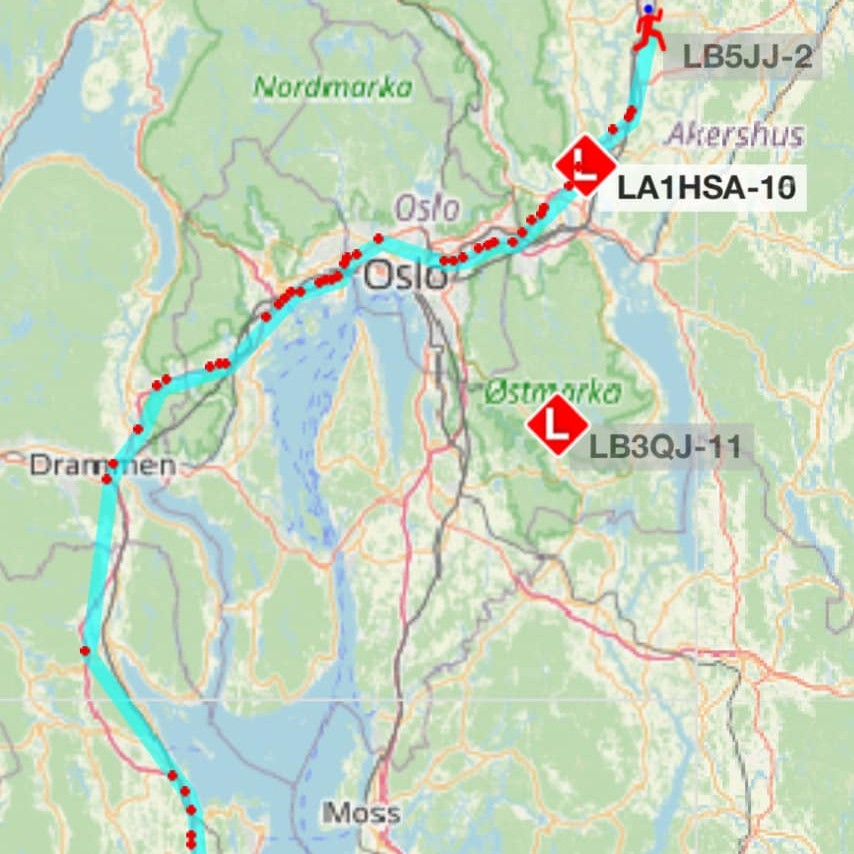
\includegraphics[width=0.8\textwidth]{aprs.jpg}
      }
    \end{column}
  \end{columns}
\end{frame}

\begin{frame}[t]
  \frametitle{Introduction to LoRa}
  \begin{columns}
    \begin{column}{0.66\textwidth}
      \begin{itemize}
        \item What is LoRa?
        \medskip
        \begin{itemize}
          \item Long Range, Low Power wireless technology
          \medskip
          \item Based on Chirp Spread Spectrum (CSS) modulation
        \end{itemize}
        \medskip
        \item LoRa Properties
        \medskip
        \begin{itemize}
          \item Long-range communication (100+ km in open areas)
          \medskip
          \item Low power consumption
        \end{itemize}
      \end{itemize}
    \end{column}
    \begin{column}{0.33\textwidth}
      \adjustbox{padding=10pt}{
        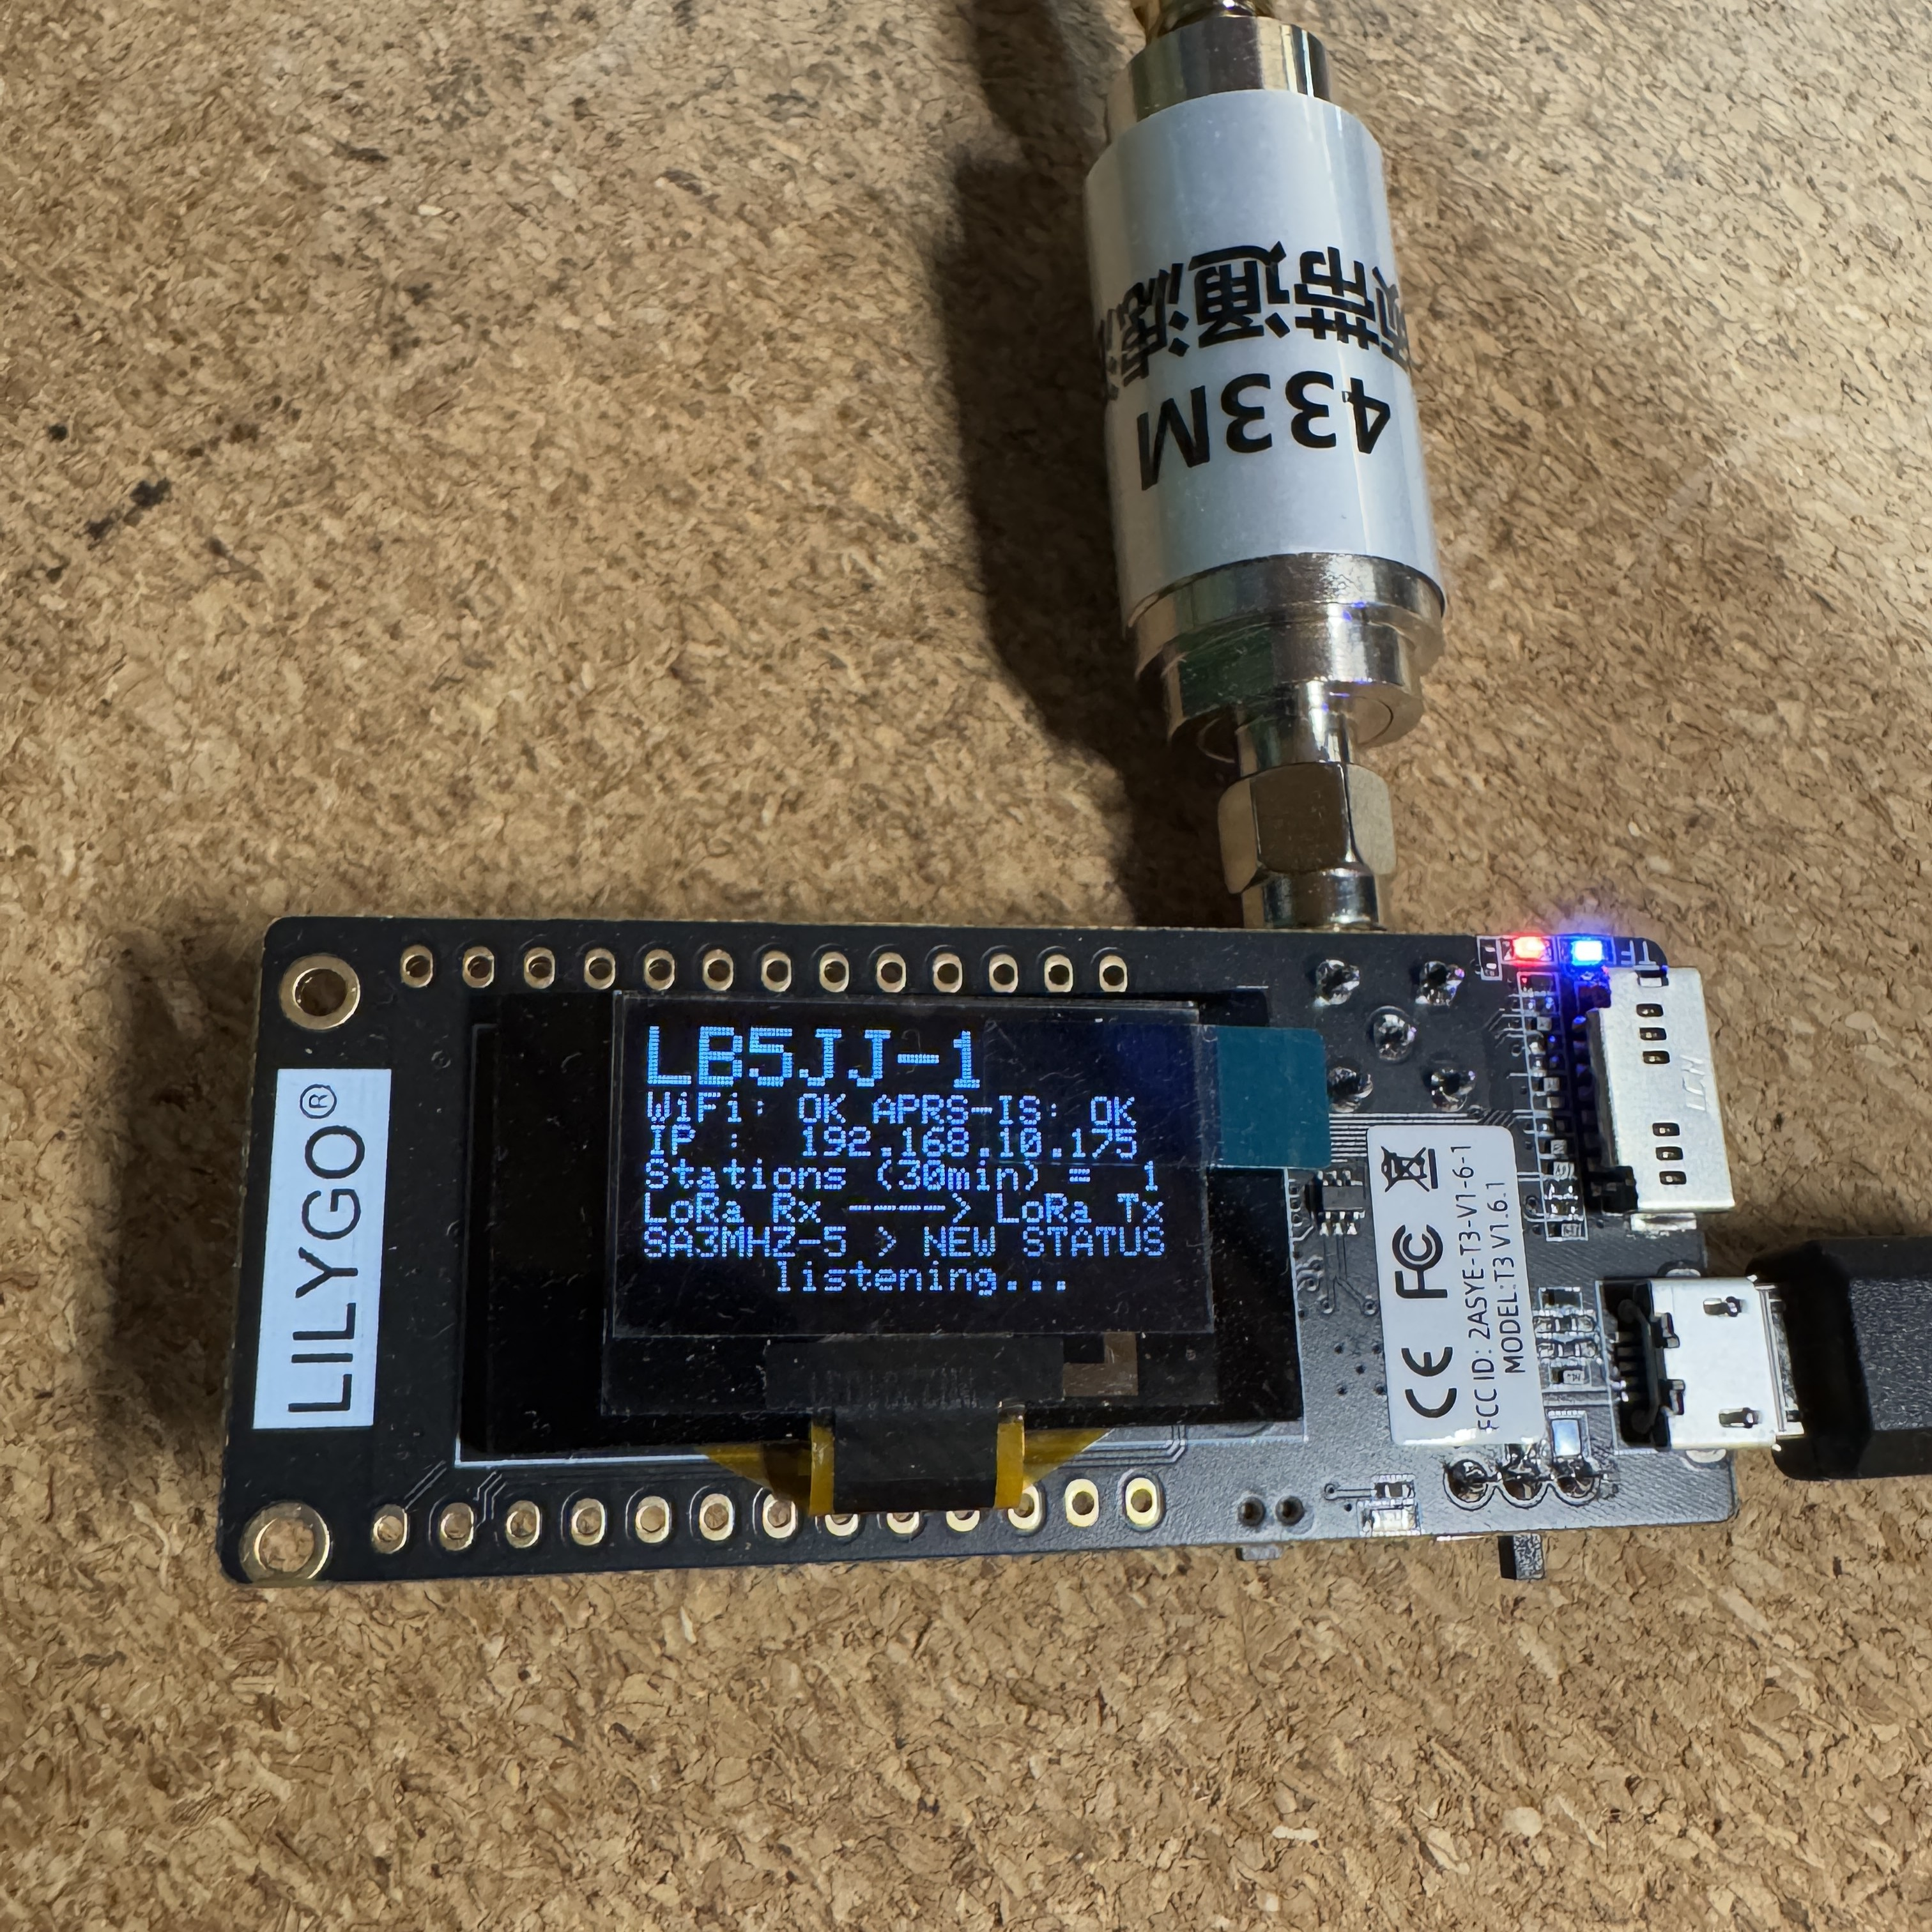
\includegraphics[width=0.8\textwidth]{lora-board.jpg}
      }
    \end{column}
  \end{columns}
\end{frame}


\begin{frame}[t]
  \frametitle{What is LoRa APRS?}
  \begin{columns}
    \begin{column}{0.66\textwidth}
      \begin{itemize}
        \item Combining LoRa and APRS
        \medskip
        \item Advantages over traditional APRS
        \medskip
        \begin{itemize}
          \item Greater range with lower power
          \medskip
          \item Suitable for modern, low-cost hardware
          \medskip
          \item Enhanced reliability in challenging environments
        \end{itemize}
      \end{itemize}
    \end{column}
    \begin{column}{0.33\textwidth}
      \adjustbox{padding=10pt}{
        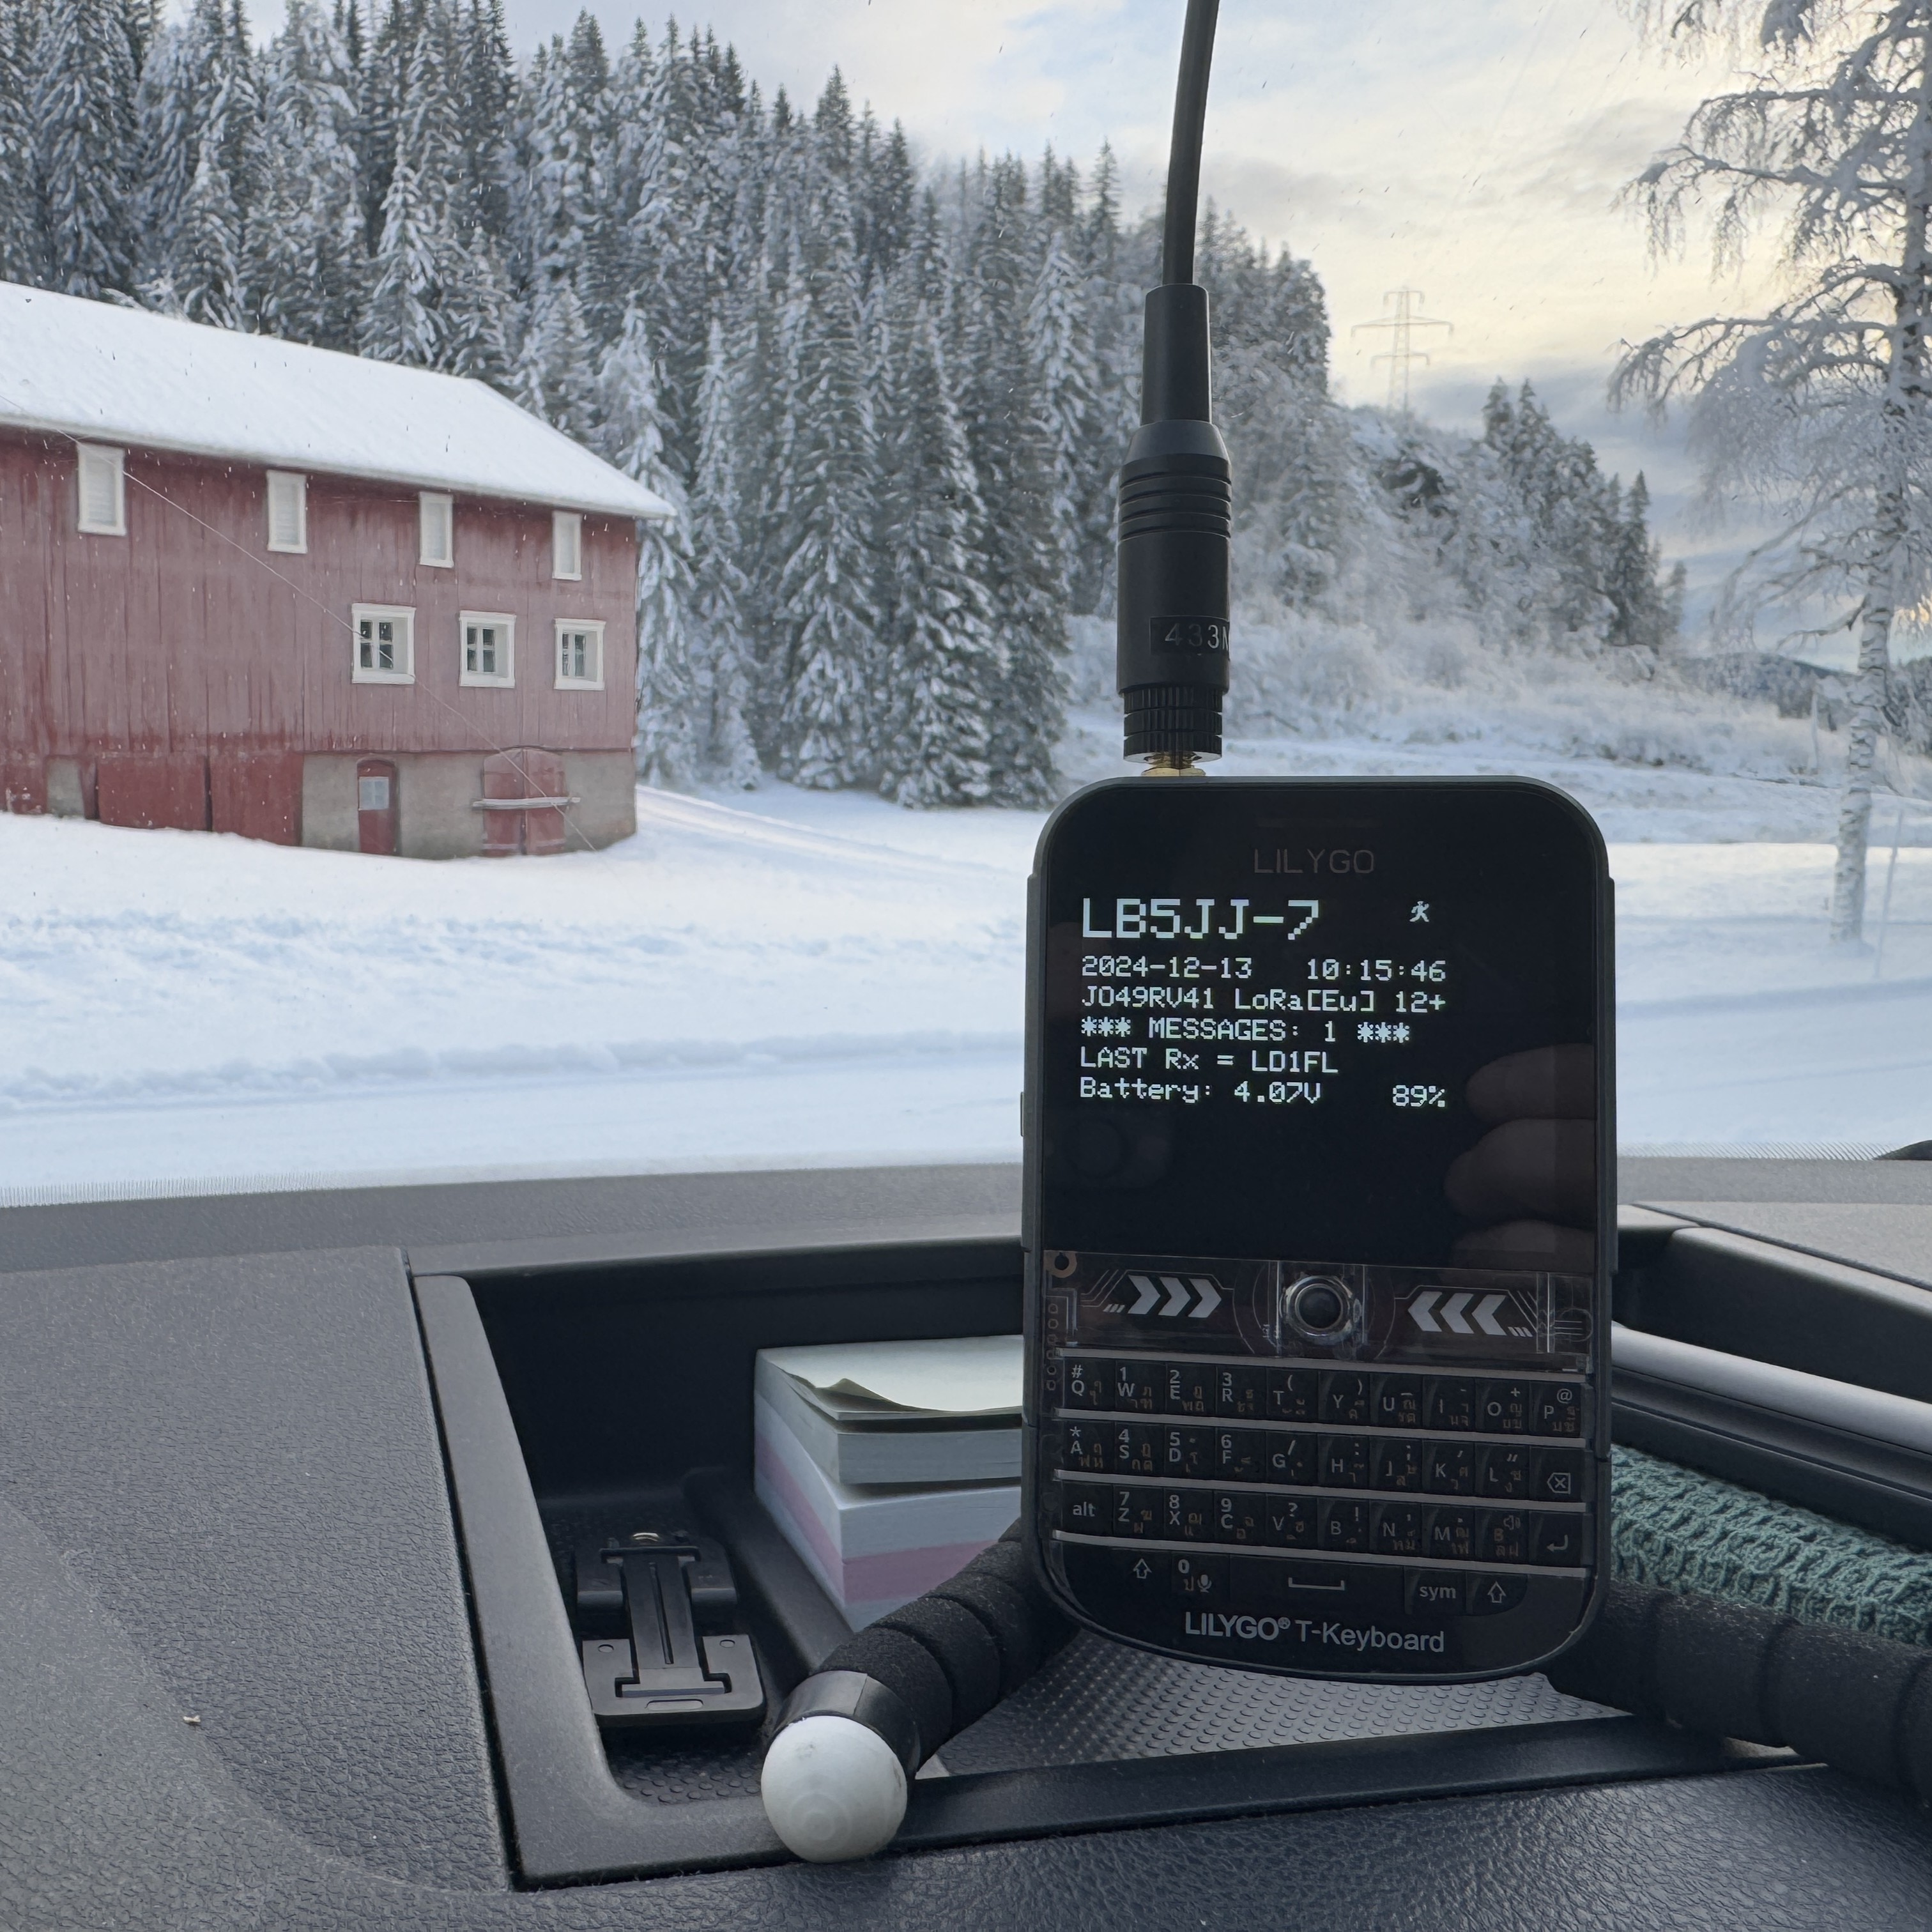
\includegraphics[width=0.8\textwidth]{t-deck-plus.jpg}
      }
    \end{column}
  \end{columns}
\end{frame}

\begin{frame}[t]
  \frametitle{Hardware}
  \begin{columns}
    \begin{column}{0.66\textwidth}
      \begin{itemize}
        \item SX1276/78
        \medskip
        \item Arduino, ESP32
        \medskip
        \item GPS receivers for position tracking
        \medskip
        \item Pre-built modules with all 3 functions on one PCB
      \end{itemize}
    \end{column}
    \begin{column}{0.33\textwidth}
      \adjustbox{padding=10pt}{
        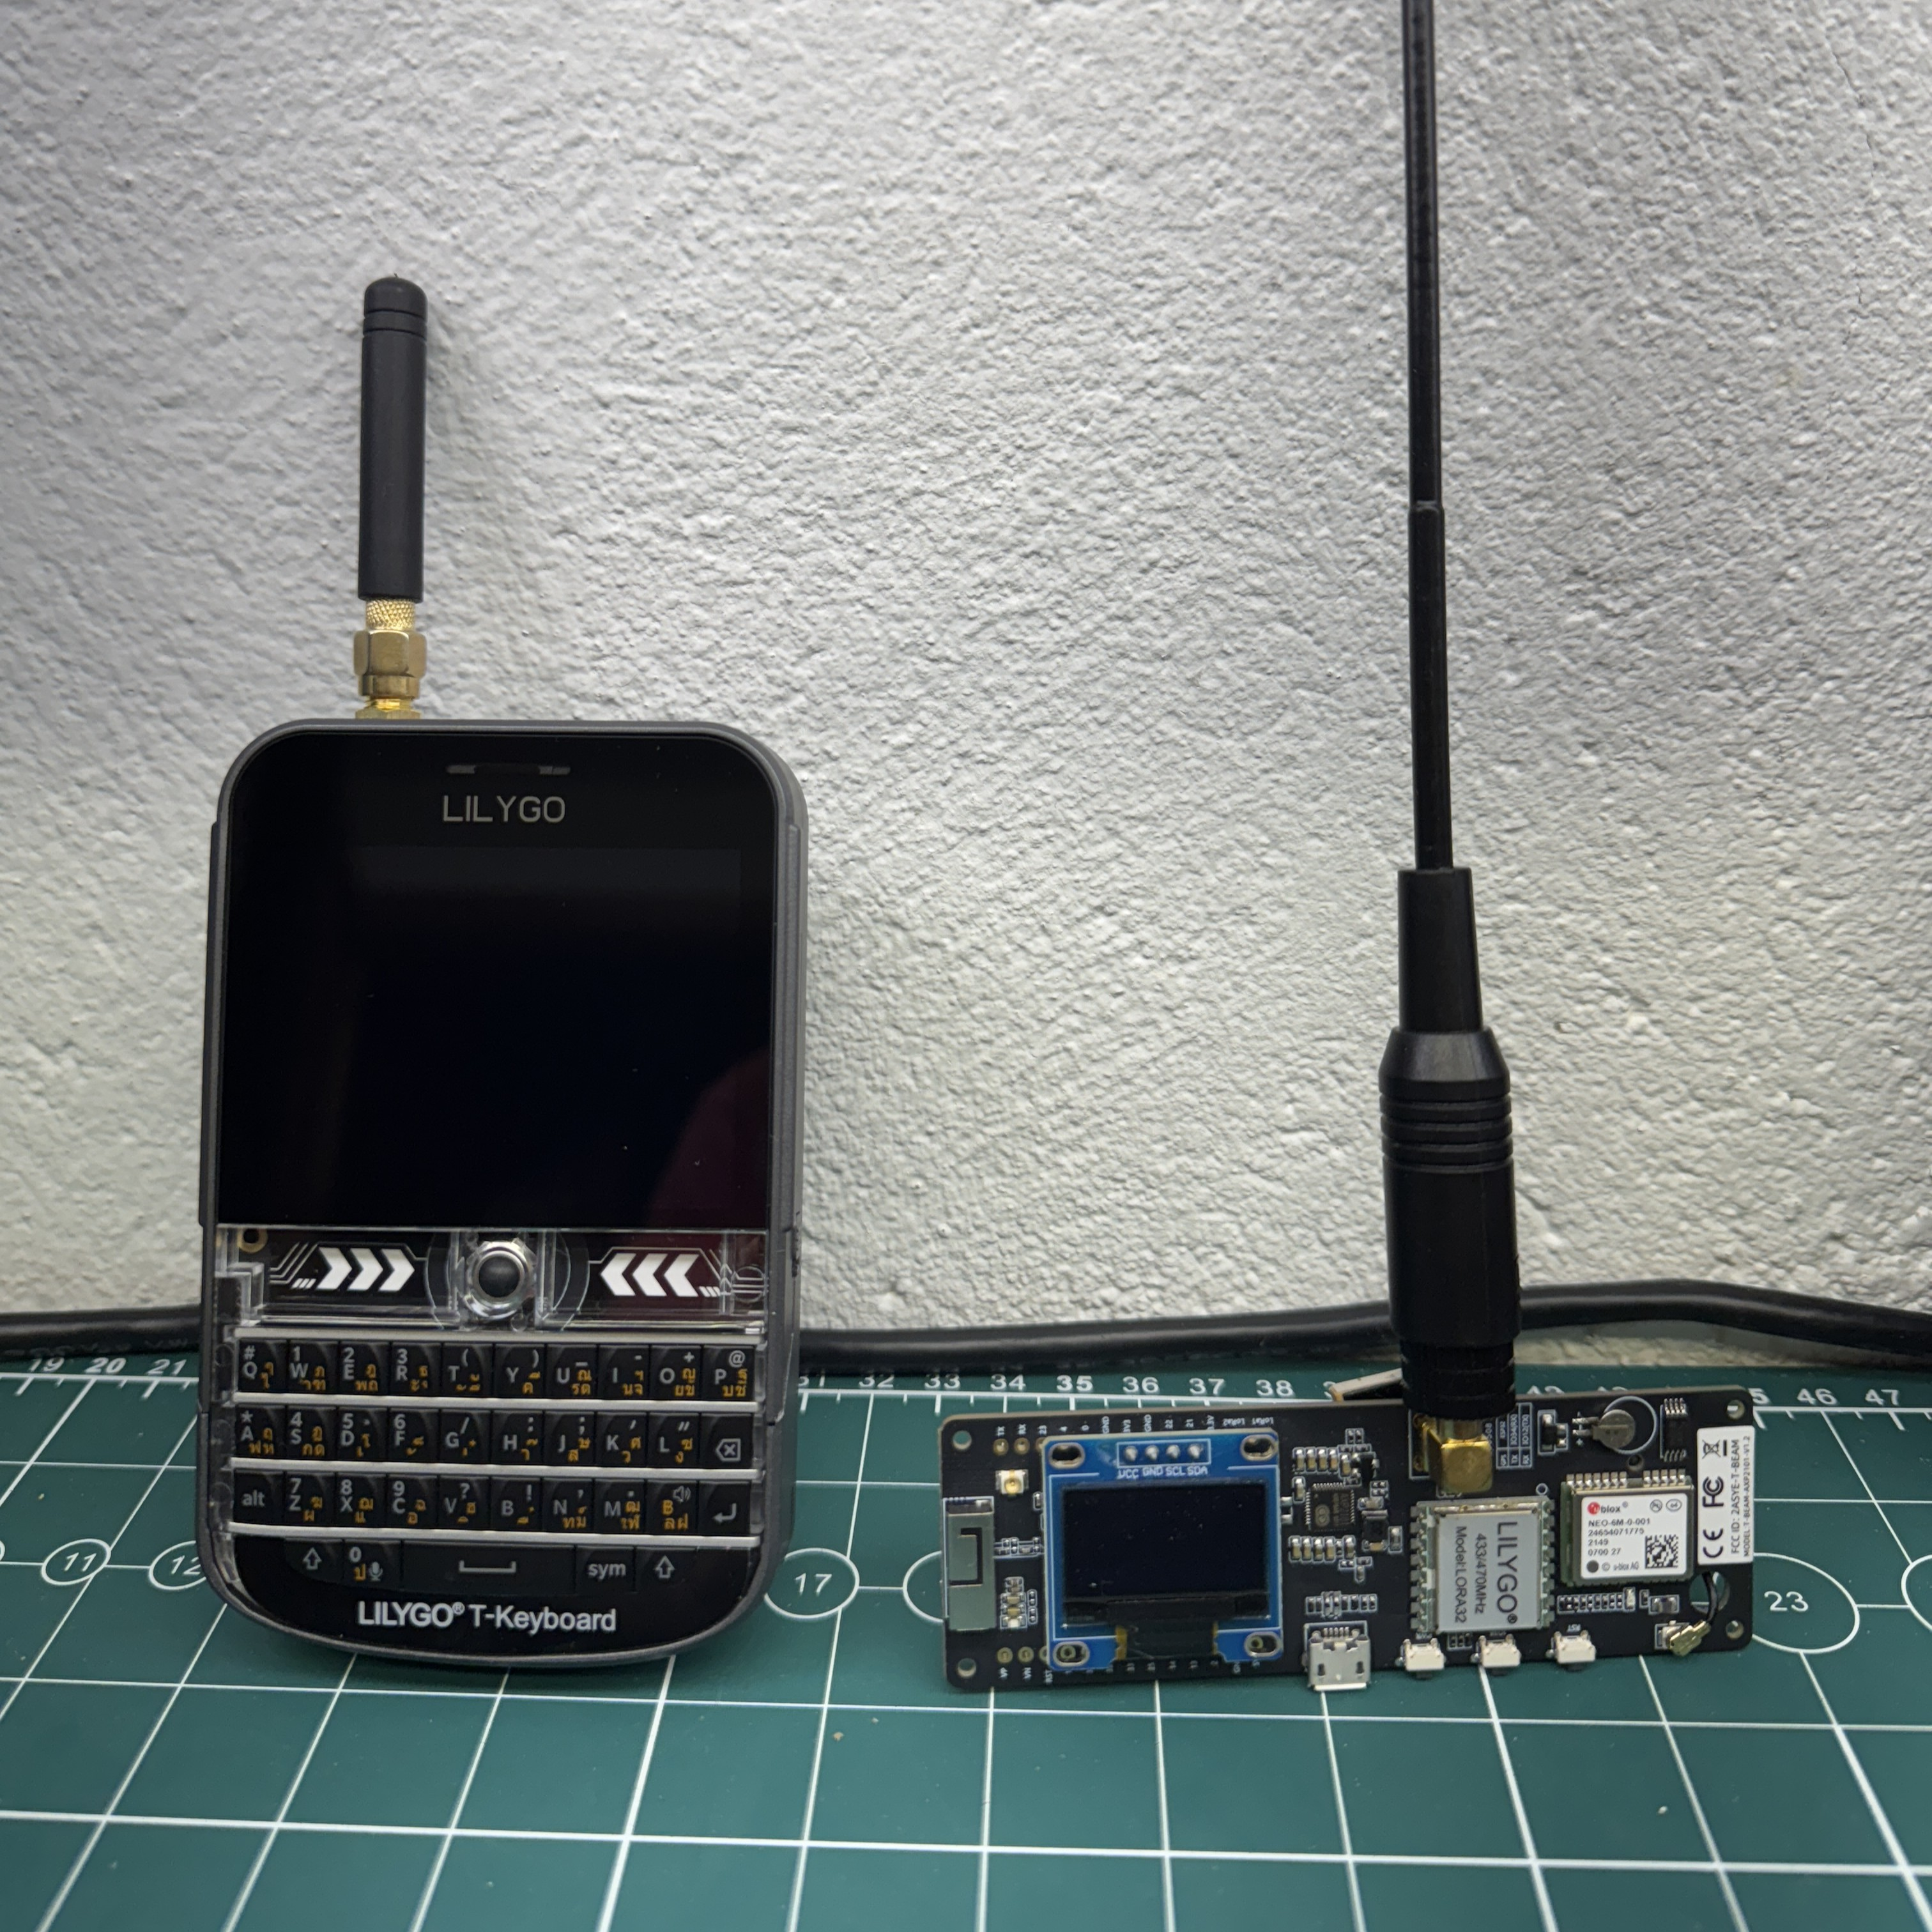
\includegraphics[width=0.8\textwidth]{hardware.jpg}
      }
    \end{column}
  \end{columns}

\end{frame}

\begin{frame}[t]
  \frametitle{Software Components}
  \begin{columns}
    \begin{column}{0.66\textwidth}
      \begin{itemize}
        \item Ricardo Guzman (CA2RXU) firmware:
        \medskip
        \begin{itemize}
          \item Tracker
          \medskip
          \item iGate/Digipeater
        \end{itemize}
        \medskip
        \item APRS.fi app for iPhone (BLE)
        \medskip
        \item APRSDroid for Android (BLE)
        \medskip
        \item PinPoint APRS for Windows (BLE, USB Serial or WiFi)
      \end{itemize}
    \end{column}
    \begin{column}{0.33\textwidth}
      \adjustbox{padding=10pt}{
        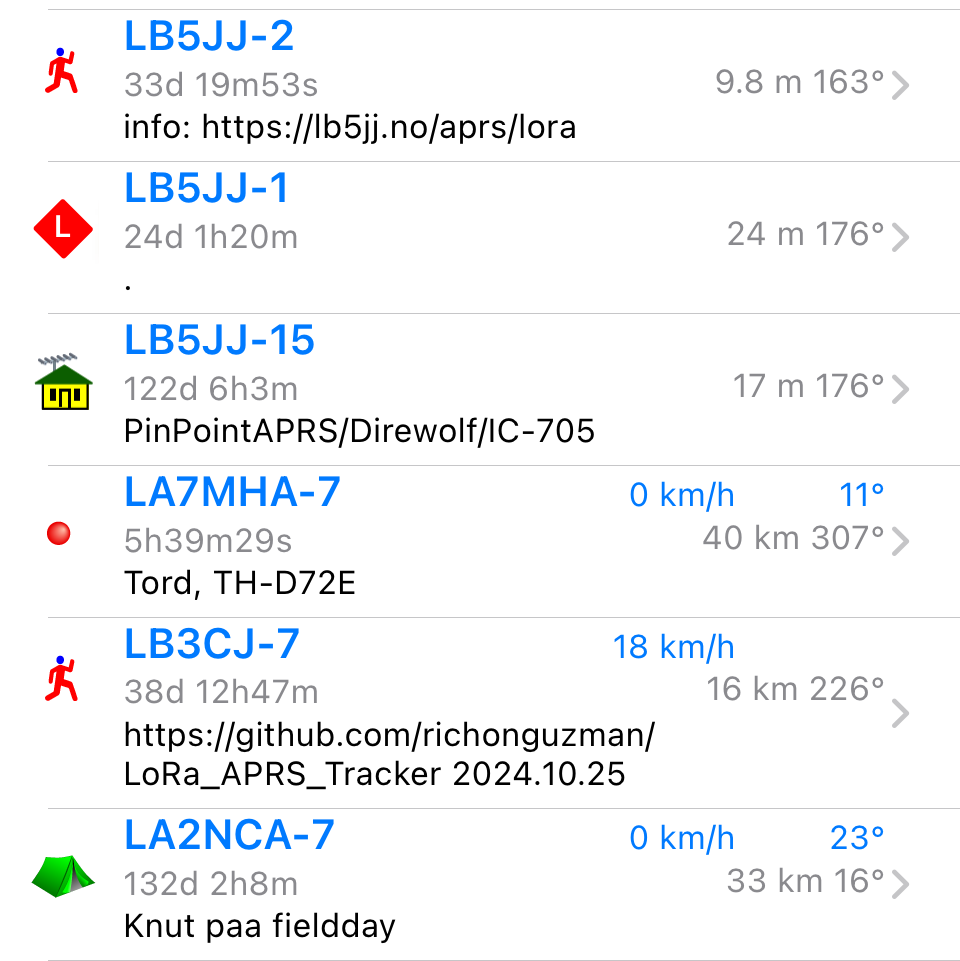
\includegraphics[width=0.8\textwidth]{software.png}
      }
    \end{column}
  \end{columns}
\end{frame}

\begin{frame}[t]
  \frametitle{How LoRa APRS Works}
  \begin{columns}
    \begin{column}{0.66\textwidth}
      \begin{itemize}
        \item Get position from GPS, or;
        \medskip
        \item Enter message on phone or keyboard
        \medskip
        \item Encode as APRS message
        \medskip
        \item Packet sent over LoRa
        \medskip
        \item Repeated by Digipeaters
        \medskip
        \item Relayed via the Internet by iGates
        \medskip
        \item Received by other LoRa APRS devices
      \end{itemize}
    \end{column}
    \begin{column}{0.33\textwidth}
      \adjustbox{padding=10pt}{
        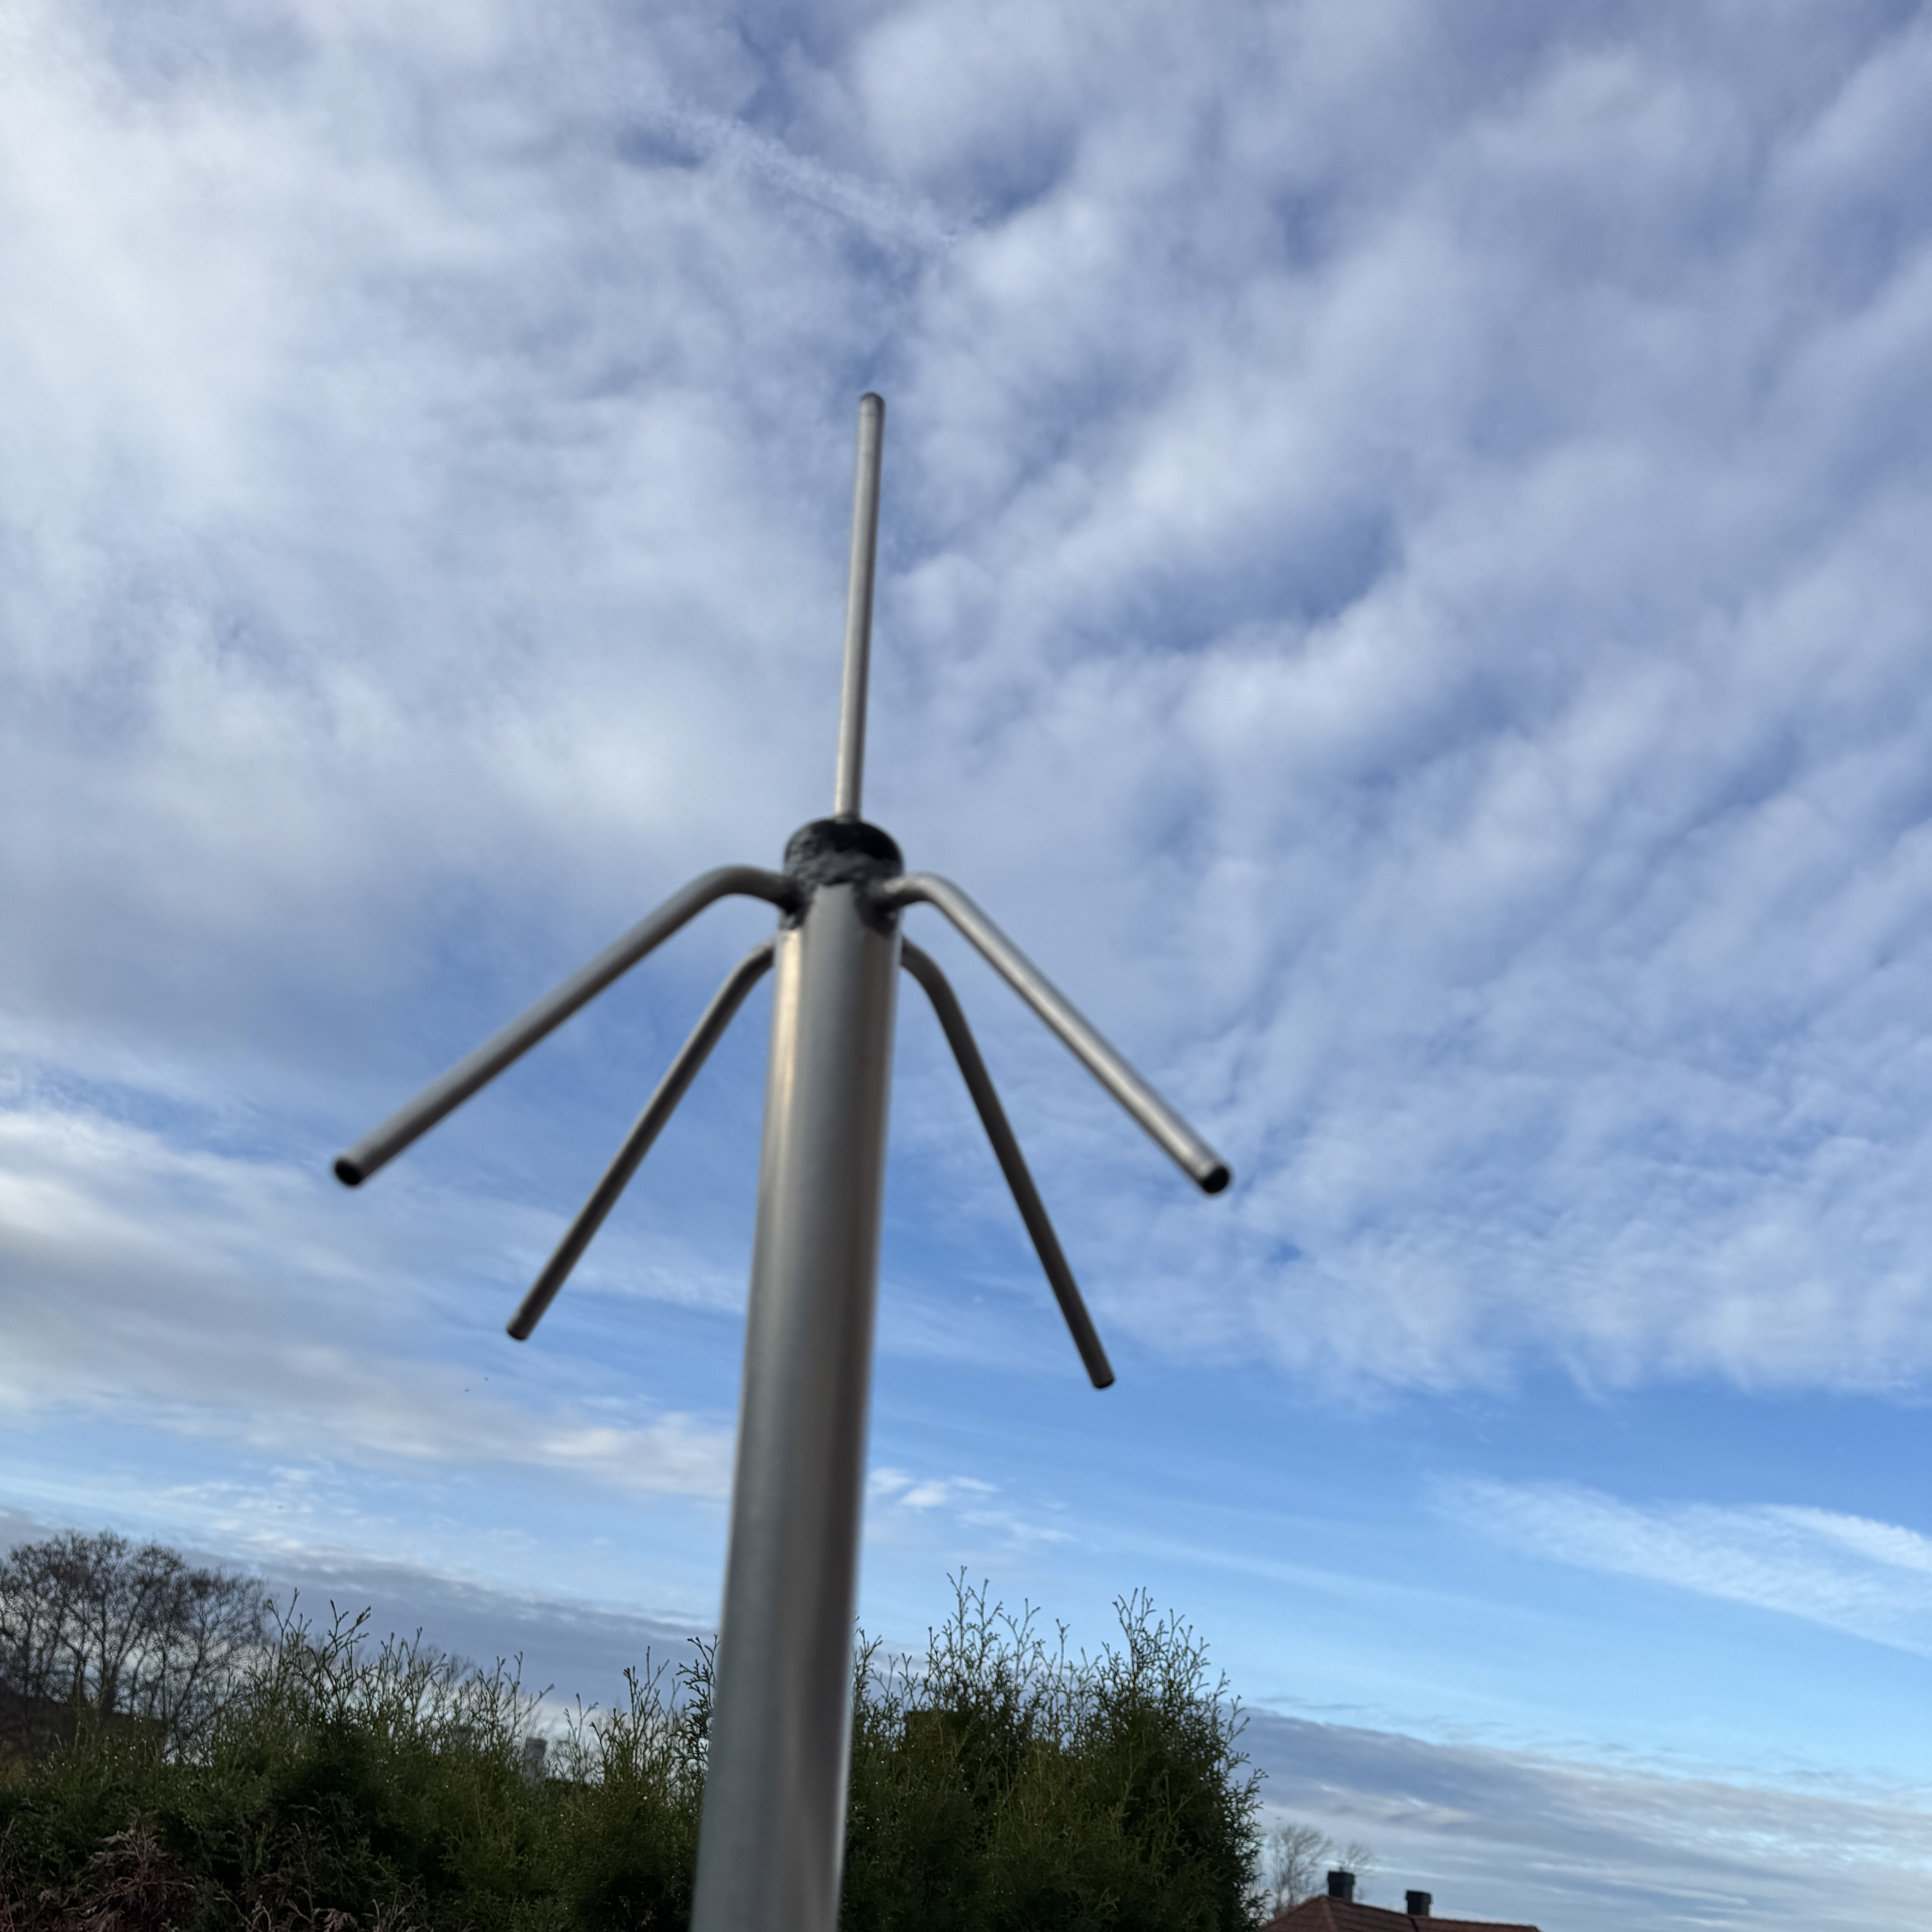
\includegraphics[width=0.8\textwidth]{antenna.jpg}
      }
    \end{column}
  \end{columns}
\end{frame}

\begin{frame}[t]
  \frametitle{Applications and Use Cases}
  \begin{columns}
    \begin{column}{0.66\textwidth}
      \begin{itemize}
        \item Adventure tracking (SOTA, POTA, Hiking)
        \medskip
        \item Off-grid messaging
        \medskip
        \item Disaster and emergency communication and tracking
        \medskip
        \item Monitoring weather stations and other sensors
        \medskip
        \begin{itemize}
          \item Alarms
          \medskip
          \item Temperature
          \medskip
          \item Battery voltage
          \medskip
          \item Others
        \end{itemize}
      \end{itemize}
      \end{column}
      \begin{column}{0.33\textwidth}
        \adjustbox{padding=10pt}{
          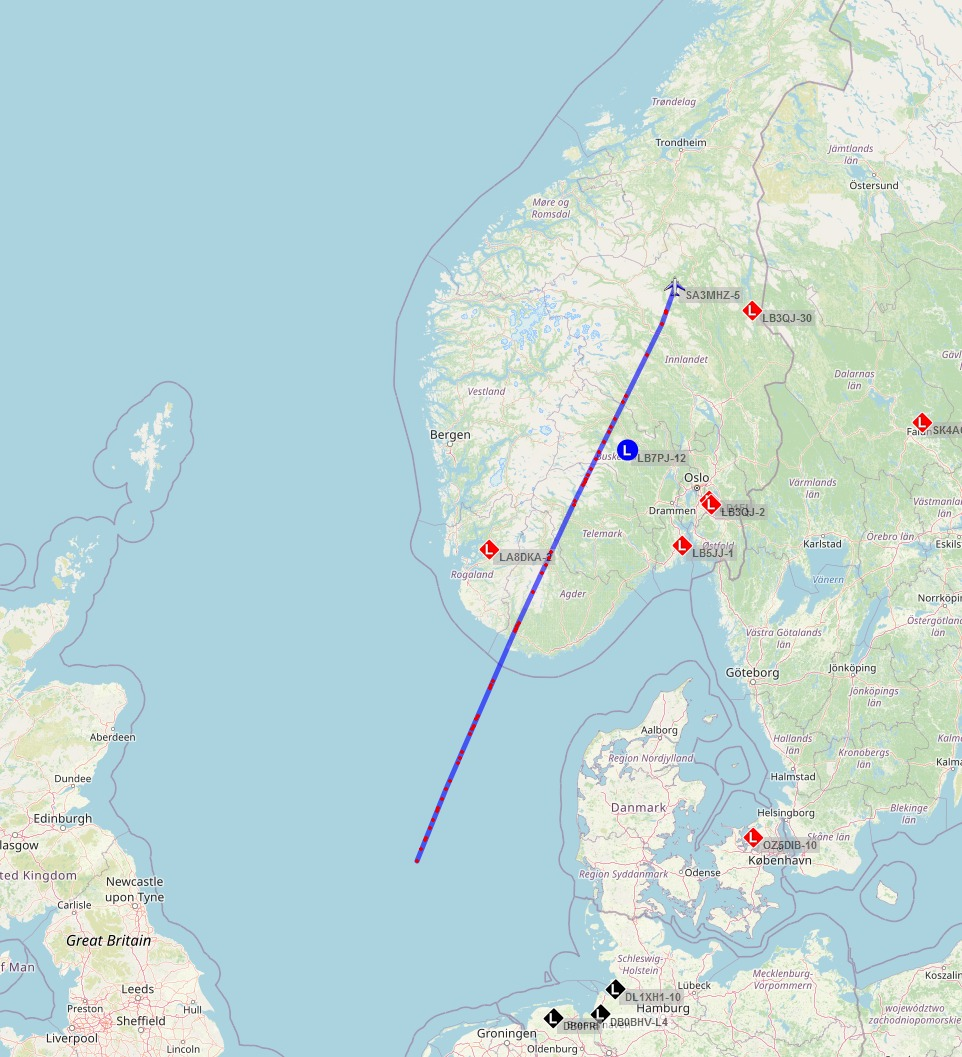
\includegraphics[width=0.8\textwidth]{tracking.jpg}
        }
      \end{column}
    \end{columns}
  \end{frame}

\begin{frame}[t]
  \frametitle{Setting Up Your LoRa APRS System}
  \begin{columns}
    \begin{column}{0.66\textwidth}
      \begin{itemize}
        \item Acquire LoRa module (eBay, AliExpress, etc)
        \medskip
        \item Install firmware (Web installer for Guzman Firmware)
        \medskip
        \item Configure (Web config for Guzman Firmware)
        \medskip
        \item Connect to APRS-IS (for iGate)
        \medskip
        \item Connect to phone / PC (Optional; for tracking / messaging)
      \end{itemize}
    \end{column}
    \begin{column}{0.33\textwidth}
      \adjustbox{padding=10pt}{
        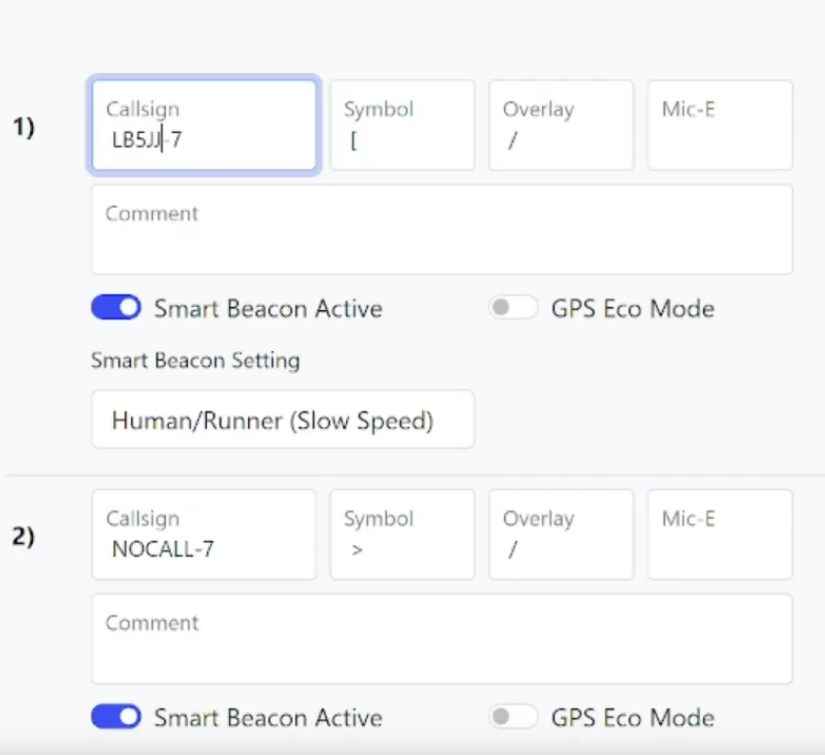
\includegraphics[width=0.8\textwidth]{install.png}
      }
    \end{column}
  \end{columns}
\end{frame}

\begin{frame}[t]
  \frametitle{Challenges and Limitations}
  \begin{itemize}
    \item Regulatory restrictions and frequency allocation
    \medskip
    \begin{itemize}
      \item Up to 200 kHz bandwidth between 433,600 og 434,000 MHz now allowed in Norway
      \medskip
      \item LoRa APRS sits on 433.775 MHz and uses 125 kHz bandwidth
      \medskip
    \end{itemize}
    \item LoRa network congestion / limited bandwidth 
    \medskip
    \begin{itemize}
      \item Only about 1/7th the transfer rate of 1200 Baud packet
      \medskip
      \item Keep your transmissions as short as possible!
    \end{itemize}
  \end{itemize}
\end{frame}

\begin{frame}[t]
  \frametitle{Links, and thanks for listening}
    \begin{itemize}
      \item \url{https://github.com/richonguzman/LoRa_APRS_Tracker}
      \medskip
      \item \url{https://github.com/richonguzman/LoRa_APRS_iGate}
      \medskip
      \item \url{https://lilygo.cc/}
      \medskip
      \item \url{https://lora-aprs.live/}
      \medskip
      \item \url{https://aprs.fi/}
      \medskip
      \item \url{https://lb5jj.no/aprs/lora/}
      \medskip
      \item cq@lb5jj.no
  \end{itemize}
\end{frame}

\end{document}